\documentclass[a4paper, 11pt]{article}

\usepackage[french]{babel}
\usepackage[T1]{fontenc}
\usepackage[utf8]{inputenc}
\usepackage{color}
\usepackage{numprint}
\usepackage{listings}

\usepackage{amssymb}
\usepackage{amsthm, thmtools}
\usepackage{amsmath}
\usepackage{amsfonts}
\usepackage{mathrsfs}
\usepackage{mathtools}
\usepackage{stmaryrd}
\usepackage{dsfont}
\usepackage[all]{xy}
\usepackage{fancyvrb}

%%%%% Configuration de listings
\lstset{
language=matlab,
basicstyle=\ttfamily\small, %
identifierstyle=\color{red}, %
keywordstyle=\color{blue}, %
stringstyle=\color{black!60}, %
commentstyle=\it\color{green!95!yellow!1}, %
columns=flexible, %
tabsize=2, %
extendedchars=true, %
showspaces=false, %
showstringspaces=false, %
numbers=left, %
numberstyle=\tiny, %
breaklines=true, %
breakautoindent=true, %
captionpos=b
}

\usepackage{xcolor}

\definecolor{Zgris}{rgb}{0.87,0.85,0.85}

\newsavebox{\BBbox}
\newenvironment{DDbox}[1]{
\begin{lrbox}{\BBbox}\begin{minipage}{\linewidth}}
{\end{minipage}\end{lrbox}\noindent\colorbox{Zgris}{\usebox{\BBbox}} \\
[.5cm]}

%%%%%%%%%%%%%%%%%%%%%%%%%%%%%%%%%%%%%%%%%%%%%%%%%%%%%%%%%%%%%%%%%%%%%%%%%%%%%%%

\usepackage{enumitem}

\usepackage{nameref, hyperref, cleveref}
	\hypersetup{
		pdfnewwindow=false,
		colorlinks=true,
		linkcolor=black,
		filecolor=black,
		urlcolor=blue,
		}

\usepackage{multicol}
	\setlength{\columnseprule}{0.1pt}
\usepackage[vmargin = 1.5cm, hmargin = 2cm]{geometry}


\newcommand{\tcr}[1]{\textcolor{red}{#1}}
\newcommand{\drond}[2]{\frac{\partial #1}{\partial #2}}
\newcommand{\R}{\mathbb{R}}
\newcommand{\Z}{\mathbb{Z}}

\renewcommand{\emph}[1]{\textbf{#1}}

\title{TP Unsupervised Learning
Compte-rendu}
\author{Antoine Moulin}
\date{}

\begin{document}

\maketitle

\section{Data}

\section{Toy examples}

La fonction $\texttt{Toy\_main.m}$ applique trois méthodes différentes ($\texttt{PCA, K-PCA \& K-means}$) à trois situations différentes : deux gaussiennes séparées, deux gaussiennes qui se recoupent et enfin le cas où les donnée sont distribuées selon deux cercles concentriques :

\begin{center}
	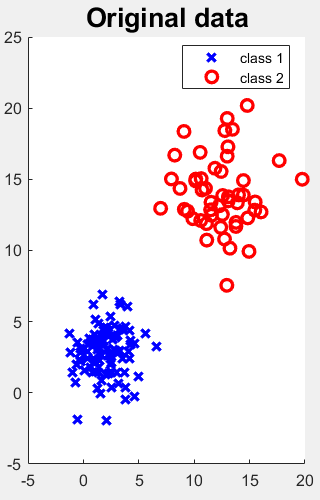
\includegraphics[scale=0.661]{separate_gaussian_dist.PNG}
	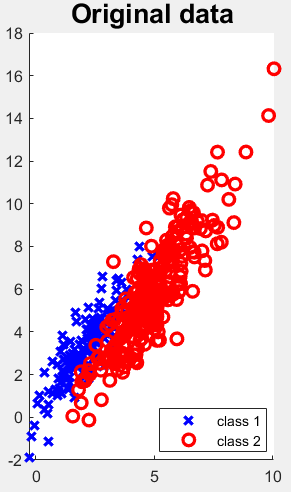
\includegraphics[scale=0.672]{overlapping_gaussian_dist.PNG}
	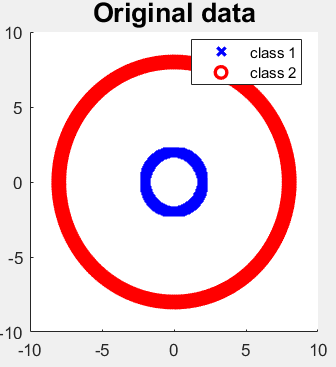
\includegraphics[scale=0.9]{circles_dist.PNG}
\end{center}

Dans le cas des deux gaussiennes séparées, les trois méthodes sont efficaces, il n'y a pas vraiment de difficulté à classer les points. Comme il s'agit de gaussiennes, la méthode \texttt{PCA} est tout à fait pertinente. On remarque d'ailleurs que la première composante principale suffit souvent à déterminer la classe d'un point. L'utilisation du kernel-trick n'est ici pas nécessaire. Concernant le clustering, il donne de bons résultats également. \\

Dans le cas de gaussiennes qui se recoupent, la \texttt{K-PCA} n'est pas vraiment efficace contrairement à la \texttt{PCA} qui semble donner de meilleurs résultats. \\

Enfin, concernant les distributions en cercles, la \texttt{PCA} ne fonctionne pas du tout. Cela vient du fait que les deux classes ne sont pas linéairement séparables. C'est pour cela qu'on utilise le kernel-trick, qui permet de plonger les données dans un espace plus grand, dans lequel les données sont séparables. C'est cette méthode qui donne les meilleurs résultats. Concernant le \texttt{K-means}, comme deux points de classes différentes peuvent être plus proches que deux points d'une même classe, il ne peut pas fonctionner non plus puisque qu'il fait en sorte de minimiser les distances intra-clusters et de maximiser les distances inter-clusters.

\section{Face recognition}

	\subsection{Goal}
	
	\subsection{PCA}
	
\begin{itemize}

	\item[1.] D'un point de vue mathématique, la formule de la matrice de covariance donnée dans le cours ne fonctionnerait pas si les données n'étaient pas centrées. Mais ça ne répond pas vraiment à la question. Il est nécessaire de centrer les données avant une \texttt{PCA} car il s'agit d'un procédé qui projette dans les directions qui maximisent la variance (formules dans le cours). De ce fait, si une feature a des valeurs bien plus élevées que les autres, elle prédominera et sera donc considérée comme une composante principale. Pour juger chaque composante de la même façon, on centre donc les données (et parfois il est préférable de les réduire également).

	\item[2.] Calculons $x_{p}x_{q}^{T}$. $U$ est une matrice orthogonale, donc $UU^{T} = I$, puis $x_{p} = y_{p}U^{T}, x_{q} = y_{q}U^{T}$. Ainsi, on a \[ x_{p}x_{q}^{T} = y_{p}U^{T} \left( y_{q}U^{T} \right)^{T} = y_{p}U^{T}U y_{q}^{T} = y_{p} y_{q}^{T} \]

i.e. \[ \boxed{x_{p}x_{q}^{T} = y_{p} y_{q}^{T}} \]

	\item[3.] La matrice de covariance
	
	\item[4.] La matrice de covariance de $Y$ est donnée par \[ \Sigma_{Y} = \frac{1}{N-1}(XU)^{T}XU = \frac{1}{N-1} U^{T}X^{T}XU = U^{T} \left( \frac{1}{N-1} X^{T}X \right) U = U^{T} C U \]
	
Or $C = UDU^{T}$, donc $U^{T}CU = D$ car $U$ est une matrice orthogonale. Ainsi, on a bien : \[ \boxed{\Sigma_{Y} = D} \]

	\item[5.] On exécute la section \texttt{PCA} de la fonction \texttt{Face\_main.m} et on trouve :
	
\begin{center}
	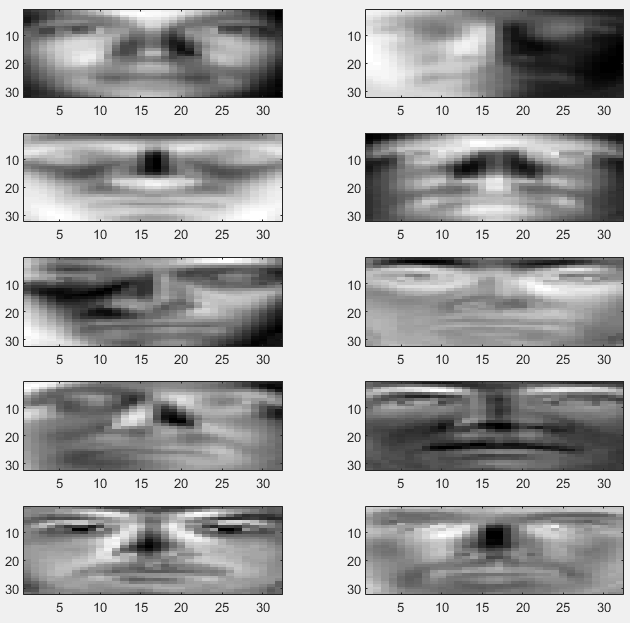
\includegraphics[scale=0.7]{eigenfaces.PNG}
\end{center}

Les visages propres ont la forme d'un véritable visage, avec des yeux, un nez, une bouche etc. En ce sens, les visages semblent réels. Il y a juste les niveaux de gris qui ne sont pas réalistes (exemple : le visage $8$ dont les sourcils sont blancs avec le reste du visage très sombre) mais certaines images pourraient faire penser à des images de vrais visages qui ont été filtrés.

	\item[6.] De façon générale, on sait que le produit vectoriel entre deux vecteurs $\textbf{u}$ et $\textbf{v}$ est donné par \[ \langle \textbf{u}, \textbf{v} \rangle = ||\textbf{u}|| \cdot ||\textbf{v}|| \cdot cos((\textbf{u}, \textbf{v})) \]
	
Ainsi, comme les deux vecteurs sont non nuls, on peut diviser par les normes et calculer l'angle : \[ \boxed{cos((\textbf{u}, \textbf{v})) = \frac{\langle \textbf{u}, \textbf{v} \rangle}{||\textbf{u}|| \cdot ||\textbf{v}||}} \]

\end{itemize}

\subsection{K-PCA}

\begin{itemize}

	\item[1.] On ne peut pas afficher les vecteurs $\left( \alpha_{i} \right)_{i}$ comme avec la \texttt{PCA} car les vecteurs $\left( \alpha_{i} \right)_{i}$ n'appartiennent pas au même espace que les données de départ (ils appartiennent à un espace de dimension plus grande).
	
	\item[2.] En utilisant le noyau gaussien (et $\sigma = 13$), on obtient les performances suivantes : 
	
\begin{center}
	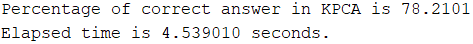
\includegraphics[scale=0.9]{kernel_gaussian_perf.PNG}
\end{center}

Avec le noyau polynomial, en prenant l'exposant égal à $4$ (semble être un bon exposant par rapport aux différentes valeurs testées), on obtient cette fois :

\begin{center}
	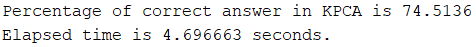
\includegraphics[scale=0.9]{kernel_poly_perf.PNG}
\end{center}

Ainsi, ce nouveau noyau semble un peu moins performant mais les résultats restent similaires.

\end{itemize}

\subsection{Performance}

\begin{itemize}

	\item[1.] Voici les résultats obtenus avec une \texttt{PCA} :
	
\begin{center}
	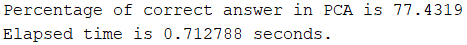
\includegraphics[scale=0.9]{pca_perf.PNG}
\end{center}

On constate donc que le \texttt{PCA} a une bien meilleure complexité que le \texttt{K-PCA}. Sous certains paramètres, on peut obtenir de meilleures résultats avec \texttt{K-PCA}, mais cette méthode est plus longue. Dans certains cas assez complexes (non linéairement séparables), il peut être préférable d'utiliser \texttt{K-PCA} comme avec l'exemple du cours. Autrement, la \texttt{PCA} semble être une bonne solution également.

	\item[2.] Bien que la méthode avec les intensités donne d'aussi bons résultats, les méthodes précédentes ont l'avantage de supprimer la redondance des données. 

\end{itemize}

\subsection{ICA and NNMF}



\section{Skin lesion segmentation}

\subsection{Goal}

\begin{itemize}

	\item[1.] A priori, il faut choisir deux classes : une pour la lésion et une pour le fond (la peau). Néanmoins, avec la présence d'autres éléments comme des poils, il peut être préférable de choisir plus de classes (par exemple 3) afin d'avoir une meilleure segmentation (car avec trois classes on aurait potentiellement une classe pour la peau, une pour la lésion et une pour les poils).
	
	\item[2.] On utilise la troisième image. Avec trois classes on obtient, pour les différents labels, les similarités suivantes :
	
\begin{center}
	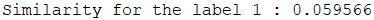
\includegraphics[scale=1]{sim_lab1.PNG} \\
	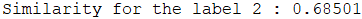
\includegraphics[scale=1]{sim_lab2.PNG} \\
	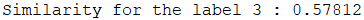
\includegraphics[scale=1]{sim_lab3.PNG}
\end{center}
	
	\item[3.] Pour choisir la classe automatiquement, on pourrait prendre celle qui maximise la similarité.

	\item[4.] En utilisant le fait que \[ (x_i  - \mu_k)^2 = \frac{1}{N_k} \sum_{j>i} z_{jk}(x_i - x_j)^2 \]
	
On a : \[ \sum_{i = 1}^N z_{ik} (x_i - \mu_k)^2 = \frac{1}{N_k} \sum_i^N z_{ik} z_{jk} \sum_{j>i} (x_i - x_j)^2 \]

puis \[ \boxed{\sum_{i = 1}^N z_{ik} (x_i - \mu_k)^2 = \frac{1}{2N_k} \sum_{i = 1}^N  \sum_{j\neq i} z_{ik} z_{jk}(x_i - x_j)^2} \]
	
	\item[5.] Une idée serait de calculer la moyenne puis de prendre l'observation la plus proche de la moyenne. Une autre méthode, peut-être un peu plus complexe utiliserait le fait suivant. Soit $ A = \lbrace a_{1}, ..., a_{n} \rbrace$ des réels. On définit $\Lambda_{A} : x \mapsto \sum_{i = 1}^{n} log(1 + |x - a_{i}|)$. On peut montrer que le minimum est nécessairement atteint en une des observations $(a_{i})_{i}$. En utilisant cette fonction au lieu de la norme euclidienne, on pourrait faire en sorte que la moyenne soit une des observations. 

\end{itemize}

\end{document}